\documentclass{article}
\usepackage{graphicx}
\usepackage{polski}
\usepackage{listings}
\usepackage{titling}
\usepackage{subcaption}
\usepackage{placeins} % Required for \FloatBarrier
\usepackage[left=3cm, right=3cm]{geometry}

\renewcommand{\lstlistingname}{Kod}

% Definicja polecenia do dodawania podtytułu

\newcommand{\subtitle}[1]{
  \posttitle{
    \par\end{center}
    \begin{center}\large#1\end{center}
    \vskip0.5em}
}
\title{Raport}
\author{Szymon Twardosz, Dominik Jeżów}
\subtitle{Permutacje macierzy i ich wpływ na kompresje}

\date{\today}

\begin{document}

\maketitle

\section{\'Srodowisko}
Do wykonania \'cwiczenia wykorzystali\'smy język
python 3.11 wraz z nast\k{e}puj\k{e}cymi bibliotekami
numpy, matplotlib, sklearn, heapq, scipy

\section{Temat zadania}

Celem zadania było wygenerowanie macierzy o rozmiarze $2^{3k}$, która opisuje topologię trójwymiarowej siatki. Po uzyskaniu macierzy, zadaniem było porównanie wzorca rzadkości tej macierzy z wzorcami powstałymi poprzez permutację źródłowej macierzy.

\noindent
Zaimplementowane przez nas metody permutacji macierzy to:
\begin{itemize}
\item Minimum degree
\item Culthill-McKee
\item Reversed Culthill-McKee
\end{itemize}

\noindent
Po przeprowadzeniu permutacji, konieczne było zbadanie efektów kompresji dla każdej z permutacji.
 macierzy.
\section{Pseudokod}
\begin{lstlisting}[language=Python, caption={Minimum degree}]
    M # macierz nXn
    G = (V, E)  #Graf eliminacji
    Permutate = [] #lista permutacji

    while not visited node in G
        from V choose p with minimal degree
        visit p
        Permutate.append(p)
        actualize G
    return Permutate
\end{lstlisting}

\begin{lstlisting}[language=Python, caption={Culthill-McKee}]
  M # macierz nXn
  G = (V, E)  #Graf eliminacji
  R = [x], where x is node with lowest degree 
  
  for i = 1,2,...
    if |R| >= n then break
    Ai = Adj(Ri) \ R #Construct the adjacency set Ai of R[i] node
    Ai.sort()
    R.append_all(Ai)
  return R
\end{lstlisting}

\begin{lstlisting}[language=Python, caption={Reversed Culthill-McKee}]
  M # macierz nXn
  G = (V, E)  #Graf eliminacji
  return reverse(Culthill-McKee(M, G))
\end{lstlisting}


\section{Ważniejsze fragmenty kodu}
\begin{lstlisting}[language=Python, caption={tworzenie grafu eliminacji}]
  def graph(matrix):
  n = len(matrix)
  V = {}
  for i in range(n):
      V[i] = set()
      for j in range(n):
          if matrix[i, j] != 0:
              V[i].add(j)
  return V
\end{lstlisting}
\begin{lstlisting}[language=Python, caption={metoda Minimum degree}]
  def minimum_degree(matrix):
      n = len(matrix)
      V = graph(matrix)
      
      pq = [(len(edge), v) for v, edge in V.items()]
      heapify(pq)
      visited = [False for i in range(n)]
      permutation = []
      
      while pq:
          _, v = heappop(pq)
          if visited[v]:
              continue
          
          visited[v] = True
          permutation.append(v)
          
          for edge in V[v]:
              if not visited[edge]:
                  V[edge].remove(v)
                  heappush(pq, (len(V[edge]), edge))
      
      return permutation  
\end{lstlisting}
\begin{lstlisting}[language=Python, caption={metoda Culthill-McKee}]
  def cuthill_mckee(matrix):
      n = len(matrix)
      V = graph(matrix) # No need to sort because I use heapque
      
      
      all_vertex = [(-len(edge), v) for v, edge in V.items()] # reverse heap
      heapify(all_vertex)
      
      bfs_pq = [all_vertex[0]]
      visited = [False for i in range(n)]
      
      permutation = []
      while bfs_pq:
          
          # If graph is no consistent - bfs_pq empty but not all vertex visited
          while not bfs_pq and all_vertex:
              _, u = heappop(all_vertex)
              if not visited[u]: heappush(bfs_pq, (-len(V[u]), u))
              
          
          _, v = heappop(bfs_pq)
          
          if visited[v]:
              continue
          
          visited[v] = True
          permutation.append(v)
          
          for edge in V[v]:
              if not visited[edge]:
                  heappush(bfs_pq, (-len(V[edge]), edge))
      
      return permutation
\end{lstlisting}
\begin{lstlisting}[language=Python, caption={metoda reversed Culthill-McKee}]
  def reversed_cuthill_mckee(matrix):
      return list(reversed(cuthill_mckee(matrix)))
\end{lstlisting}
\section{Wyniki}

\subsection{Wzorce rzadkości macierzy}
\FloatBarrier
\begin{figure}[htbp]
  \centering
  \begin{subfigure}[b]{0.4\textwidth}
      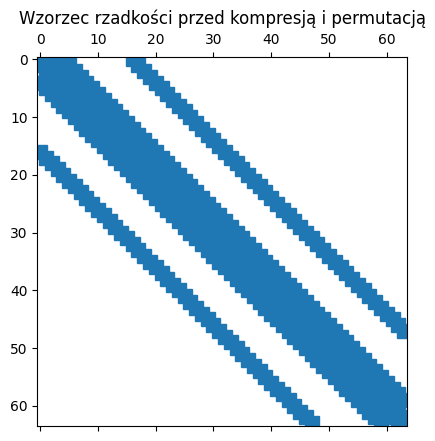
\includegraphics[width=\linewidth]{img/2ak2.png}
      \caption{k=2}
      \label{fig:obraz1}
  \end{subfigure}
  \hfill
  \begin{subfigure}[b]{0.4\textwidth}
      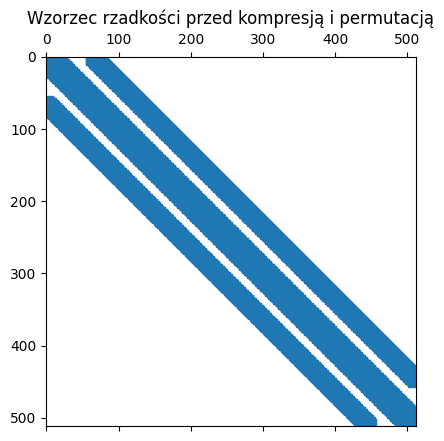
\includegraphics[width=\linewidth]{img/2ak3.png}
      \caption{k=3}
      \label{fig:obraz2}
  \end{subfigure}
  \caption{Macierz orginalna dla różnych k}
  \label{fig:zestaw_obrazkow}
\end{figure}

\FloatBarrier
Dla zadanej klasy macierzy wejściowych, metoda permutacji "minimal degree" wykazuje odzwierciedlenie identycznościowe. To niepożądane zjawisko oznacza, że permutacja ta nie wprowadza istotnej zmiany w strukturze macierzy, zachowując jej podstawowe właściwości. Jest to problematyczne, gdyż celem permutacji jest zazwyczaj wprowadzenie pewnego stopnia rzadkości lub innego ułatwienia algorytmicznego, co w przypadku odzwierciedlenia identycznościowego nie zostaje osiągnięte.
\begin{figure}[htbp]
  \centering
  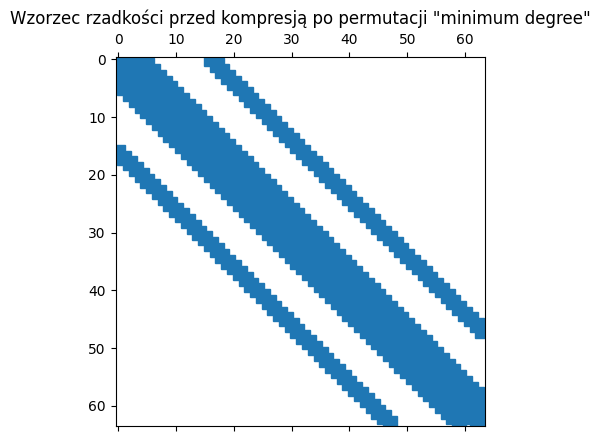
\includegraphics[width=0.9\textwidth]{img/2c1k2.png}
  \caption{permutacja minimal degree}
\end{figure}
\FloatBarrier
\begin{figure}[htbp]
  \centering
  \begin{subfigure}[b]{0.4\textwidth}
      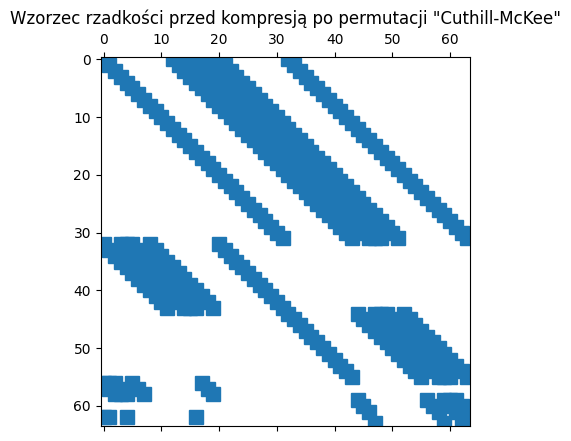
\includegraphics[width=\linewidth]{img/2c2k2.png}
      \caption{k=2}
      \label{fig:obraz1}
  \end{subfigure}
  \hfill
  \begin{subfigure}[b]{0.4\textwidth}
      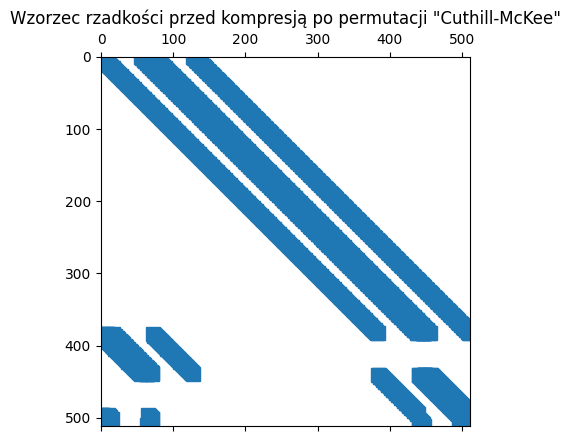
\includegraphics[width=\linewidth]{img/2c2k3.png}
      \caption{k=3}
      \label{fig:obraz2}
  \end{subfigure}
  \caption{permutacje Culthill-McKee}
  \label{fig:zestaw_obrazkow}
\end{figure}
\FloatBarrier
\begin{figure}[htbp]
  \centering
  \begin{subfigure}[b]{0.4\textwidth}
      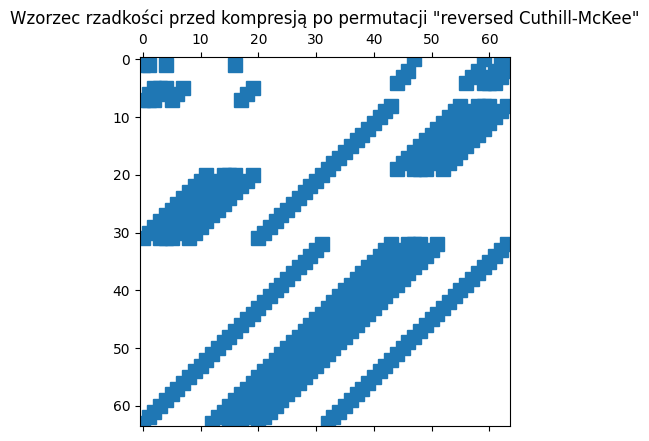
\includegraphics[width=\linewidth]{img/2c3k2.png}
      \caption{k=2}
      \label{fig:obraz1}
  \end{subfigure}
  \hfill
  \begin{subfigure}[b]{0.4\textwidth}
      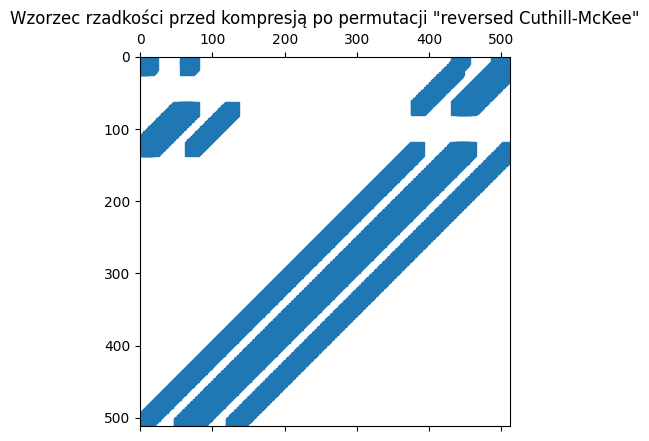
\includegraphics[width=\linewidth]{img/2c3k3.png}
      \caption{k=3}
      \label{fig:obraz2}
  \end{subfigure}
  \caption{permutacje reversed Culthill-McKee}
  \label{fig:zestaw_obrazkow}
\end{figure}
\FloatBarrier


Po obserwacji rysunków 3 i 4 można zauważyć, że dla mniejszych wartości k większa procentowa część została poddana permutacji.
% --------------------------------------------------------------------------

\begin{figure}[htbp]
  \subsection{Kompresja SVD}
  \centering
  \begin{subfigure}[b]{0.4\textwidth}
      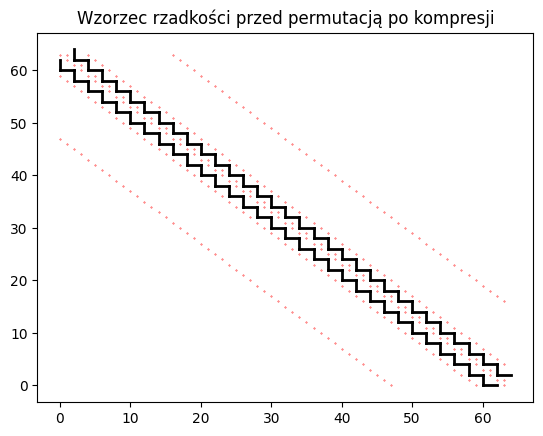
\includegraphics[width=\linewidth]{img/2bk2.png}
      \caption{k=2}
      \label{fig:obraz1}
  \end{subfigure}
  \hfill
  \begin{subfigure}[b]{0.4\textwidth}
      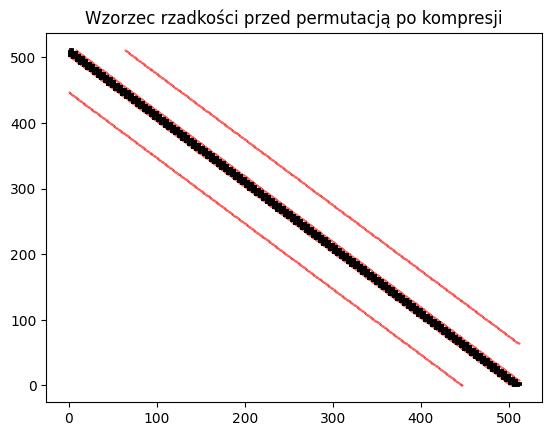
\includegraphics[width=\linewidth]{img/2bk3.png}
      \caption{k=3}
      \label{fig:obraz2}
  \end{subfigure}
  \caption{Kompresja SVD macierzy orginalnej}
  \label{fig:zestaw_obrazkow}

  \raggedright
  Zauważalne jest, że dla mniejszych wartości k znacznie bardziej wyraziste stają się obszary macierzy poddane kompresji. Dla przypadku k=3, na przekątnej widoczna jest czarna linia, wskazująca na liczne, mniejsze kompresje w tym obszarze.

  Ponadto, zauważalne jest, że nie udało się skompresować macierzy we wszystkich miejscach.
\end{figure}




\FloatBarrier
\begin{figure}[htbp]
  \centering
  \begin{subfigure}[b]{0.4\textwidth}
      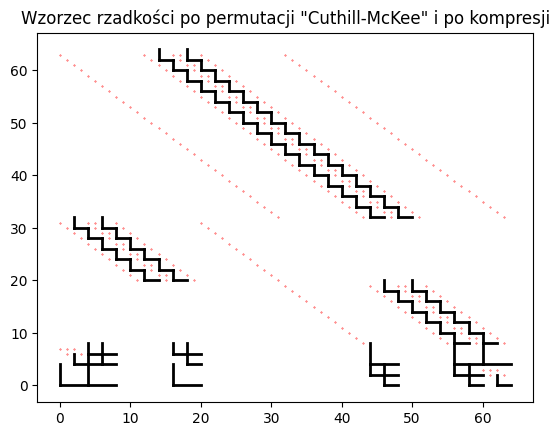
\includegraphics[width=\linewidth]{img/2d2k2.png}
      \caption{k=2}
      \label{fig:obraz1}
  \end{subfigure}
  \hfill
  \begin{subfigure}[b]{0.4\textwidth}
      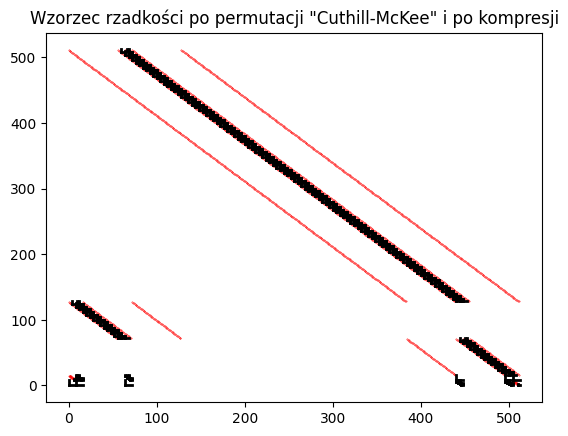
\includegraphics[width=\linewidth]{img/2d2k3.png}
      \caption{k=3}
      \label{fig:obraz2}
  \end{subfigure}
  \caption{kompresjia po urzyciu metody Culthill-McKee}
  \label{fig:zestaw_obrazkow}
\end{figure}
\FloatBarrier
\begin{figure}[htbp]
  \centering
  \begin{subfigure}[b]{0.4\textwidth}
      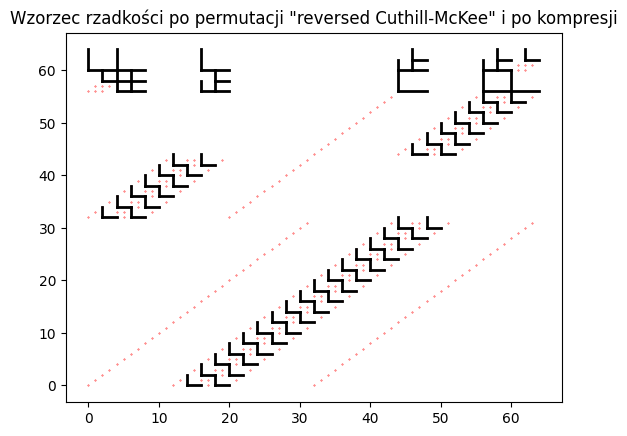
\includegraphics[width=\linewidth]{img/2d3k2.png}
      \caption{k=2}
      \label{fig:obraz1}
  \end{subfigure}
  \hfill
  \begin{subfigure}[b]{0.4\textwidth}
      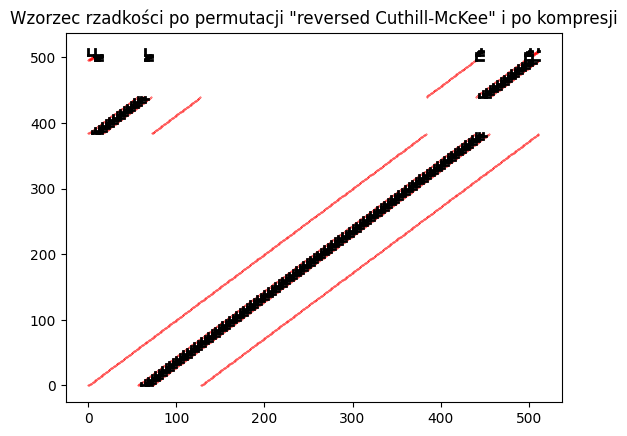
\includegraphics[width=\linewidth]{img/2d3k3.png}
      \caption{k=3}
      \label{fig:obraz2}
  \end{subfigure}
  \caption{kompresjia po urzyciu metody reversed Culthill-McKee}
  \label{fig:zestaw_obrazkow}
\end{figure}

Po zastosowaniu metod typu Culthill-McKee zauważalne są większe, oddzielone obszary, które zostały skompresowane. Ponadto, zauważamy większą ilość obszarów, które uległy kompresji (w dolnej części rysunku można dostrzec znacznie mniejszą liczbę czerwonych punktów).
\FloatBarrier

\section{Wnioski}
\begin{itemize}
  \item Metoda permutacji "Minimum degree" okazała się bezużyteczna dla podanej klasy macierzy.
  \item Metody "Culthill-McKee" oraz "reversed Culthill-McKee" prowadzą do leprzej kompresji
  \item Macierz uzyskana za pomocą metody "reversed Culthill-McKee" wygląda jak ta po zastosowaniu "Culthill-McKee" obrócona o $180^{\circ}$
  \item Można zauważyć że dla mniejszego k większa częśc macierzy została przepermutowana.
\end{itemize}
\end{document}